\documentclass{beamer}
\usetheme{default}
\useoutertheme{miniframes}
\useinnertheme{circles}
\usepackage{listings}
\usepackage{xcolor}
\usepackage{bookmark}
\usepackage{url}
\usepackage{xurl}
\usepackage{graphicx}

% =============================================
% COLOR SCHEME: Professional Navy
% =============================================
\definecolor{NavyDark}{RGB}{20, 40, 80}        % Deep navy
\definecolor{NavyMid}{RGB}{40, 65, 115}        % Medium navy
\definecolor{NavyLight}{RGB}{70, 100, 150}     % Lighter navy accent

% Set the main structure color
\setbeamercolor{structure}{fg=NavyDark}

% Header (top navigation bar)
\setbeamercolor{section in head/foot}{fg=white, bg=NavyDark}
\setbeamercolor{subsection in head/foot}{fg=white, bg=NavyMid}

% Footer colors (subtle gradient)
\setbeamercolor{author in head/foot}{fg=white, bg=NavyLight}
\setbeamercolor{title in head/foot}{fg=white, bg=NavyMid}
\setbeamercolor{date in head/foot}{fg=white, bg=NavyDark}

% Title page
\setbeamercolor{title}{fg=NavyDark}
\setbeamercolor{subtitle}{fg=NavyMid}
\setbeamercolor{author}{fg=NavyDark!80}
\setbeamercolor{date}{fg=NavyDark!60}

% Frame titles
\setbeamercolor{frametitle}{fg=white, bg=NavyDark}
\setbeamercolor{framesubtitle}{fg=white}

% Itemize/enumerate colors
\setbeamercolor{item}{fg=NavyDark}
\setbeamercolor{subitem}{fg=NavyMid}

% Navigation dots
\setbeamercolor{mini frame}{fg=white, bg=white!30}
\setbeamercolor{mini frame inactive}{fg=white!50}

% Custom footline: Author | Short Title | Date + Frame Number
\setbeamertemplate{footline}{
  \leavevmode%
  \hbox{%
  \begin{beamercolorbox}[wd=.20\paperwidth,ht=2.5ex,dp=1ex,left,leftskip=1em]{author in head/foot}%
    \usebeamerfont{author in head/foot}\insertshortauthor
  \end{beamercolorbox}%
  \begin{beamercolorbox}[wd=.55\paperwidth,ht=2.5ex,dp=1ex,center]{title in head/foot}%
    \usebeamerfont{title in head/foot}\insertshorttitle
  \end{beamercolorbox}%
  \begin{beamercolorbox}[wd=.25\paperwidth,ht=2.5ex,dp=1ex,right,rightskip=1em]{date in head/foot}%
    \usebeamerfont{date in head/foot}\insertshortdate{}\hspace*{2em}
    \insertframenumber{} / \inserttotalframenumber
  \end{beamercolorbox}}%
  \vskip0pt%
}

% Code listing style
\lstset{
    basicstyle=\ttfamily\footnotesize,
    breaklines=true,
    frame=single,
    backgroundcolor=\color{gray!10},
}

\title[Systems Thinking Workshop Series \#2: Gen AI Workflows]{Systems Thinking for Better Science \#2: \\ \textbf{Introduction to Gen AI Workflows}}
\subtitle{\textbf{Setting Aside the Hype and the Fear, and Getting Started}}
\author[Sneha]{\textbf{Sneha} (sneha@artpark.in)}
\date[16 Apr 2026]{16 Apr 2026\\[0.6em]{\tiny Link to presentation: \url{https://github.com/dsih-artpark/workshops/blob/main/workshops/workshop-02-gen-ai-workflows-01/presentation.pdf}}}

\begin{document}

\maketitle


% =============================================
% OPENING
% =============================================
\section{Opening}

% Slide 2: Interactive opener
% Facilitator: ask the question, invite 2-3 people to briefly share their incident,
% acknowledge the range of what you hear (wins, disasters, both), then move to the spiral
\begin{frame}{}
\begin{center}
\Large
Raise your hand if AI has surprised you - in either direction.

\end{center}
\end{frame}

% Slide 3: The spiral
% Facilitator: "here's a frame for everything you just heard"
% NOTE: save the Liz Fosslien spiral image to this folder as spiral.png
\begin{frame}{}
\begin{center}
    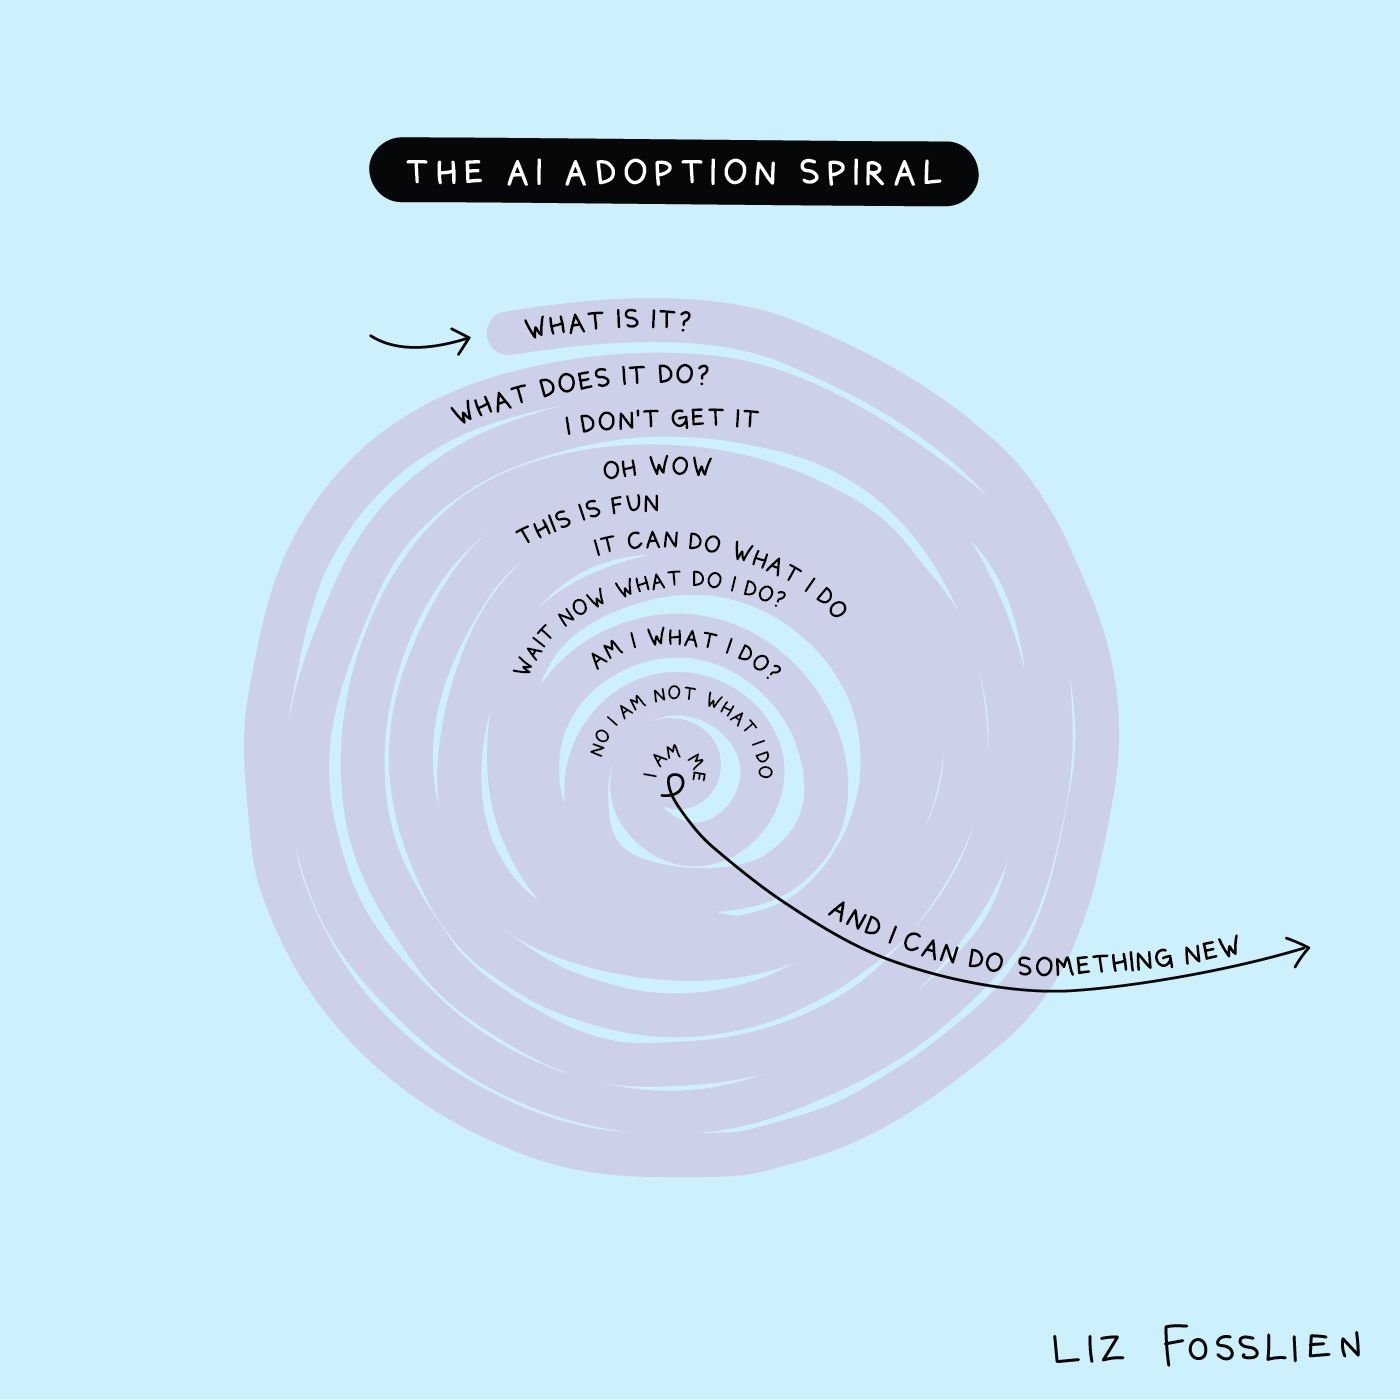
\includegraphics[width=0.62\textwidth]{spiral.png}

    \vspace{0.3em}
    {\tiny Liz Fosslien [1]}
\end{center}
\end{frame}

% Slide 4: The comparison reframe
% Facilitator: hold the pause after this lands
\begin{frame}{}
\begin{center}
\Large
Everyone on this spiral thinks everyone else is further along.
\break

\pause
\Large
Trust me, I'm NOT an expert either. I just like yapping.
\end{center}
\end{frame}

% Slide 5: Normalise the disorientation
\begin{frame}{This Isn't Specifically an AI Problem}
New technology has always felt this way.

\vspace{1em}
The spiral isn't a sign that something is wrong with you or the tools.
It's the emotional arc of every significant shift in how we work.

\vspace{1.5em}
\textit{So you have to first navigate your relationship with your work before you jump to the next step.}
\end{frame}

% Slide 6: Industry context - framed as normalisation, not a scorecard
\begin{frame}{Even Start Ups and Enterprises Are Still Figuring It Out}
\textbf{The scale of adoption:}
\begin{itemize}
    \item Ramp: 99.5\% of their team on AI tools, usage up 6,300\% year-on-year [2]
    \item Shopify's CEO made AI proficiency a performance expectation for every employee [3]
\end{itemize}

\vspace{1em}
\textbf{What that's also produced:}
\begin{itemize}
    \item Amazon's main shopping site went down for six hours following AI-assisted code changes [4]
    \item 40\% of workers have received AI-generated content that looks polished but communicates nothing - each instance costs roughly 2 hours to resolve [5]
\end{itemize}

\vspace{0.8em}
\textit{The confusion is rational. Especially at the frontier, this is hard.}
\end{frame}

\begin{frame}{At the centre of all this is also}

\pause
\begin{itemize}
    \item    A massive hype engine on Social Media
    \pause
    \item    Which in turn drives major fears - fear of missing out, fear of being left behind
\end{itemize}

\end{frame}

% Slide 7: Transition
\begin{frame}{Where do we start today?}

\normalsize
The best way to fight overwhelm is with systems. And a plan.

\normalsize
\pause
\vspace{1em}
\small
Three rules of thumb to get started:
\vspace{1em}
\pause
\begin{enumerate}
    \item Think First
    \pause
    \item Ask Plainly
    \pause
    \item Iterate Recursively
    \pause
        \begin{enumerate}
            \item Iterate Recursively
            \pause
                \begin{enumerate}
                \item Iterate Recursively
                \pause
                \item And take it one step at a time.
                \end{enumerate}
        \end{enumerate}
\end{enumerate}


\vspace{0.6em}

\pause
\break
Disclaimer: This talk contains what I've derived from my readings and experiences. \only<9->{YMMV\footnote{Your mileage may vary.}.}
\end{frame}


% =============================================
% SECTION 1: THINK FIRST, THEN DELEGATE
% =============================================
\section{Think First}

\begin{frame}{\#1: Think First, Then Delegate}
Start from what the consumer of your content \textit{(i.e. the user)} actually needs before you start delegating.
\pause

\vspace{0.8em}
Clarify the job: e.g. Slack \& Sophie Alpert [6].

\pause
\vspace{0.8em}
If you don't clarify your work and go in to the task confused, AI will amplify that confusion. Because it is fundamentally trained on the "average" of all work that's out there. 
\pause
Lack of guidance will produce an average work - and poor guidance can even produce less than average work.

\pause
\vspace{0.8em}
\textit{The thinking is the work. Delegation comes after. Think of AI as a talented junior you can delegate work to. She's talented, but she's a junior.}
\end{frame}

\begin{frame}{The Original Slack Flowchart}
\begin{center}
    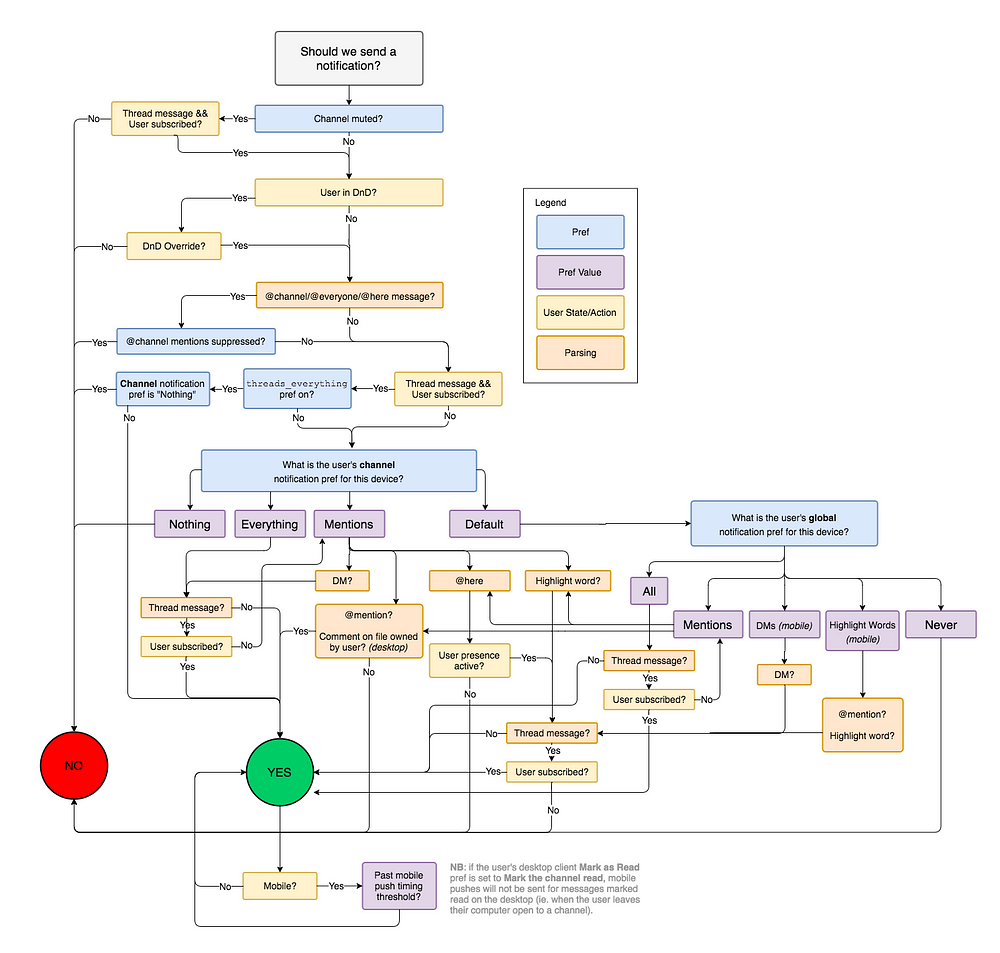
\includegraphics[height=0.72\textheight, width=\textwidth, keepaspectratio]{slack-original.png}

    \vspace{0.3em}
    {\tiny Slack, via Sophie Alpert [6]}
\end{center}
\end{frame}

\begin{frame}{After: Starting From What the User Actually Wants}
\begin{center}
    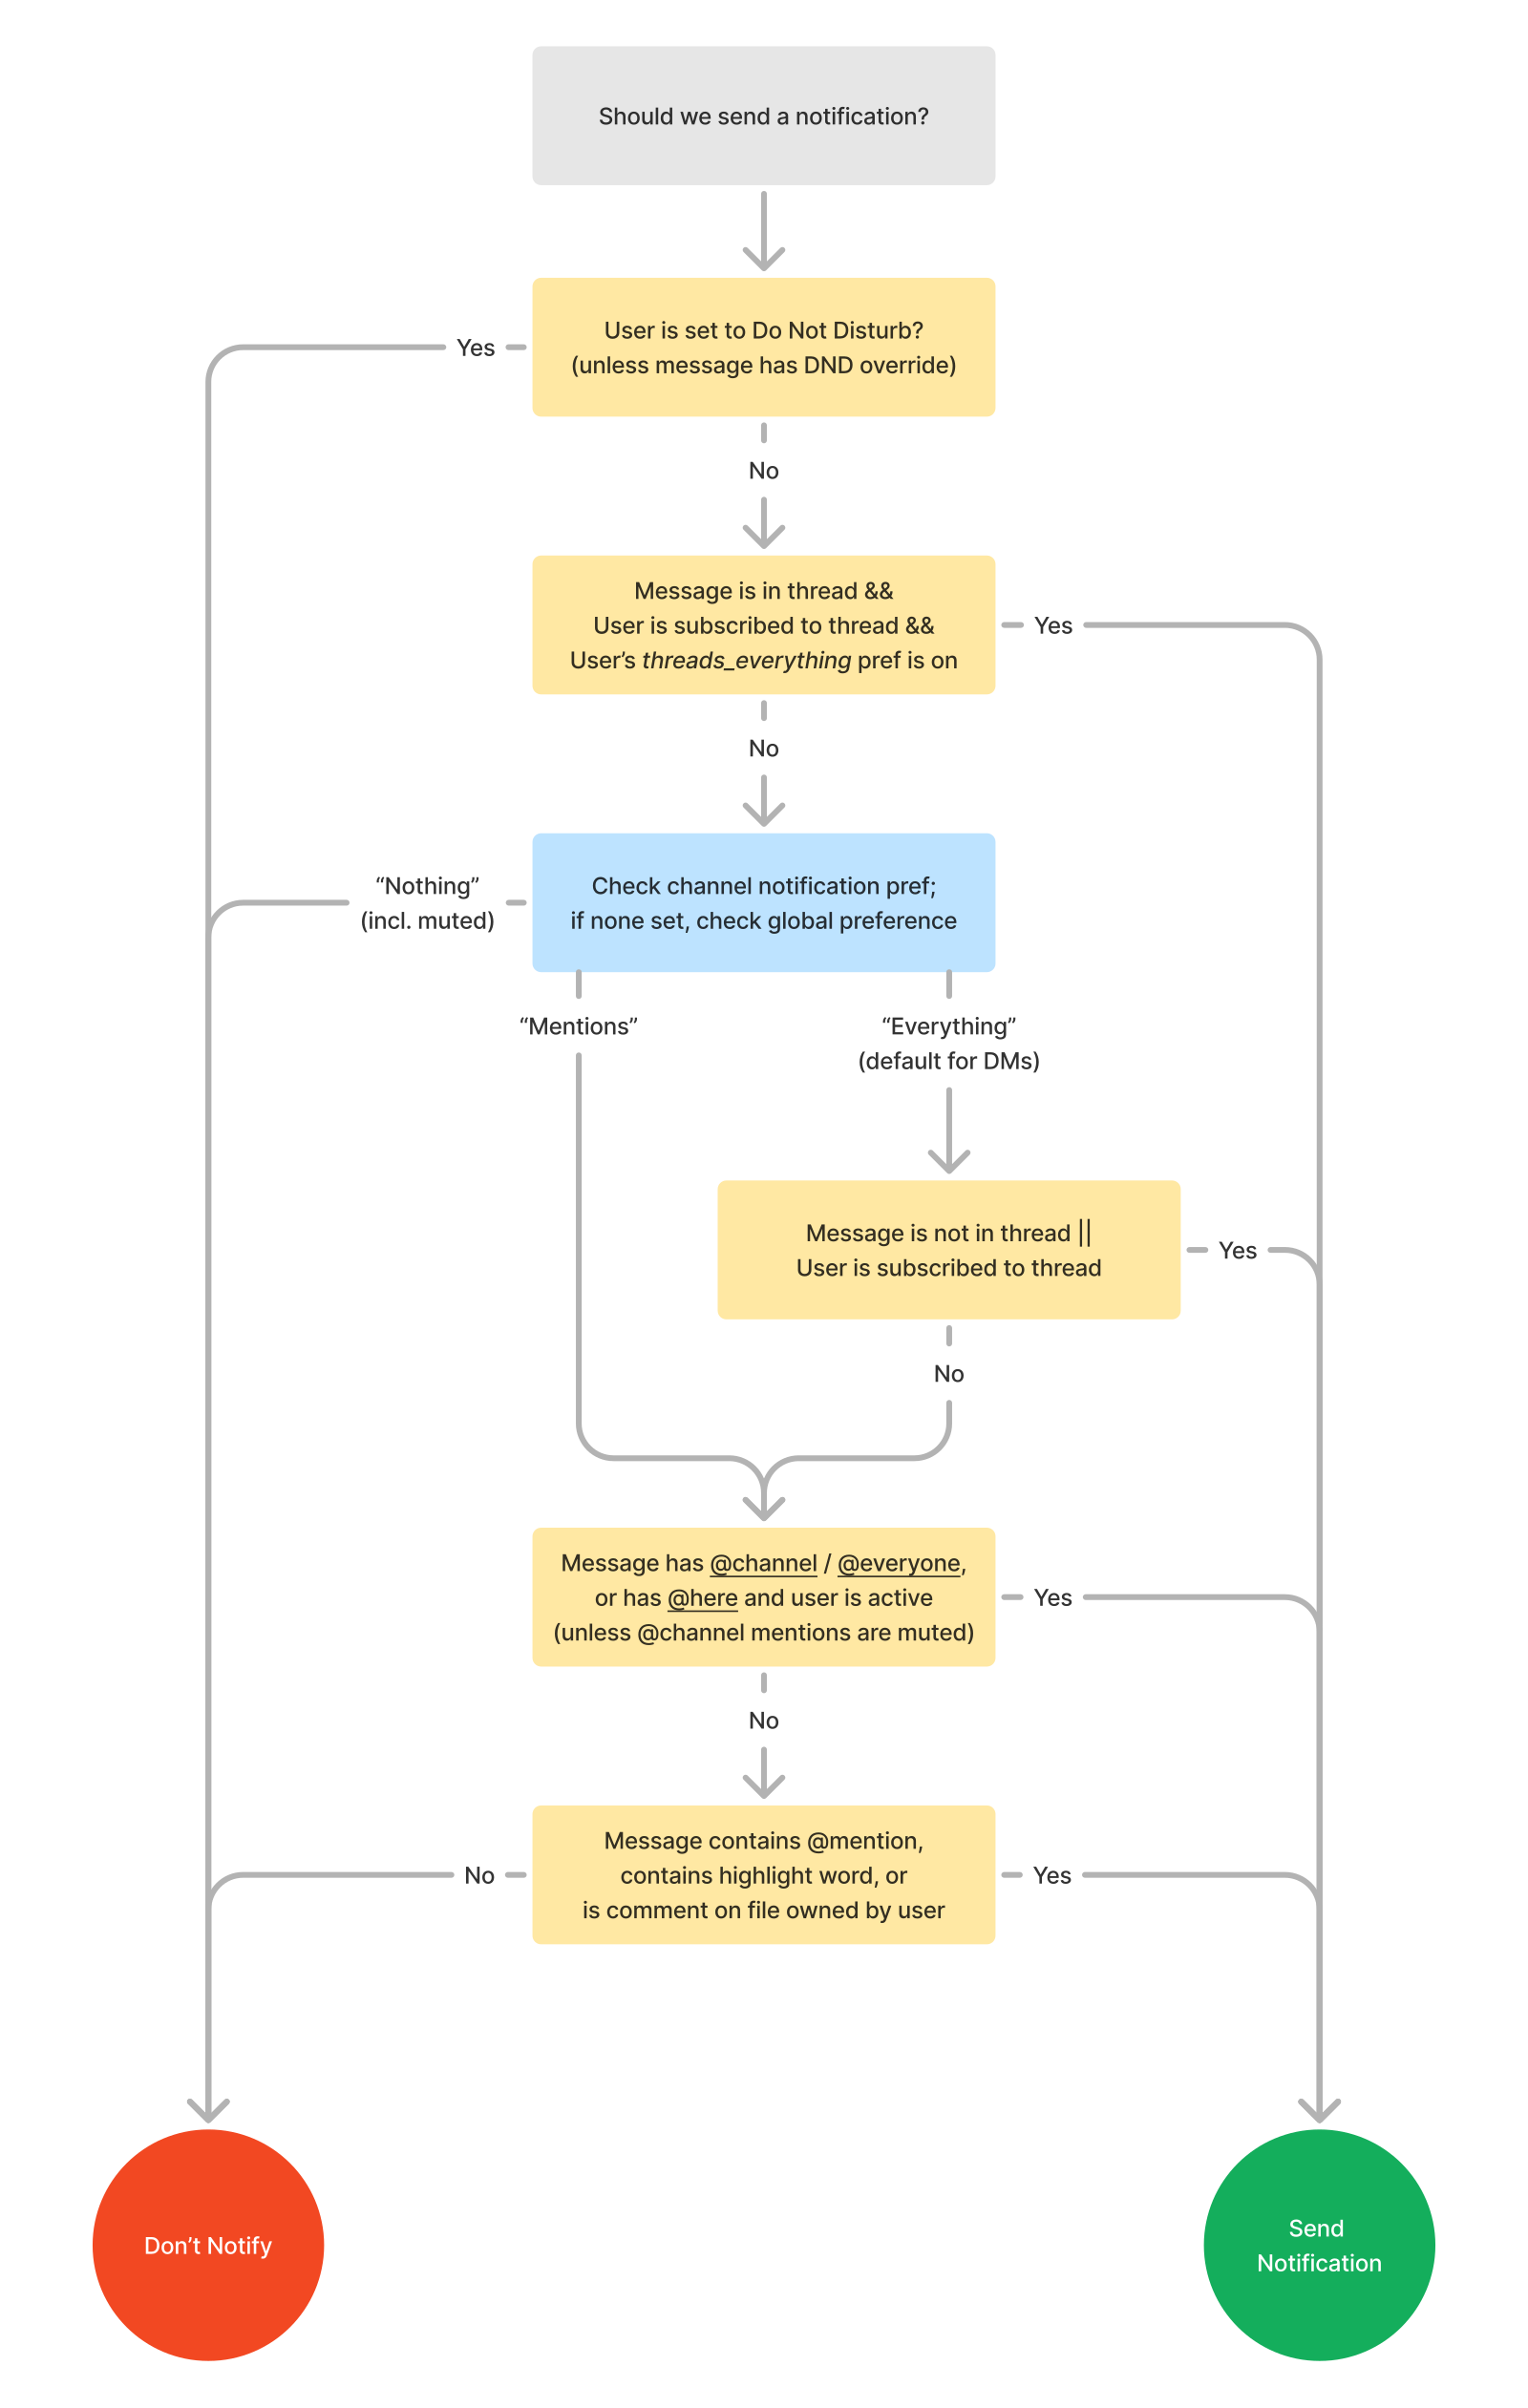
\includegraphics[height=0.66\textheight, width=\textwidth, keepaspectratio]{slack-simplified.png}

    \vspace{0.3em}
    {\tiny Sophie Alpert [6]}
\end{center}

\vspace{0.2em}
{\footnotesize\textit{Next move: once the thinking is clear, the asking can be plain.}}
\end{frame}


\section{Ask Plainly}

\begin{frame}{Simpler Inputs Work Better Over Time}
\framesubtitle{KISS: Keep it Simple, Stupid}
\begin{center}
    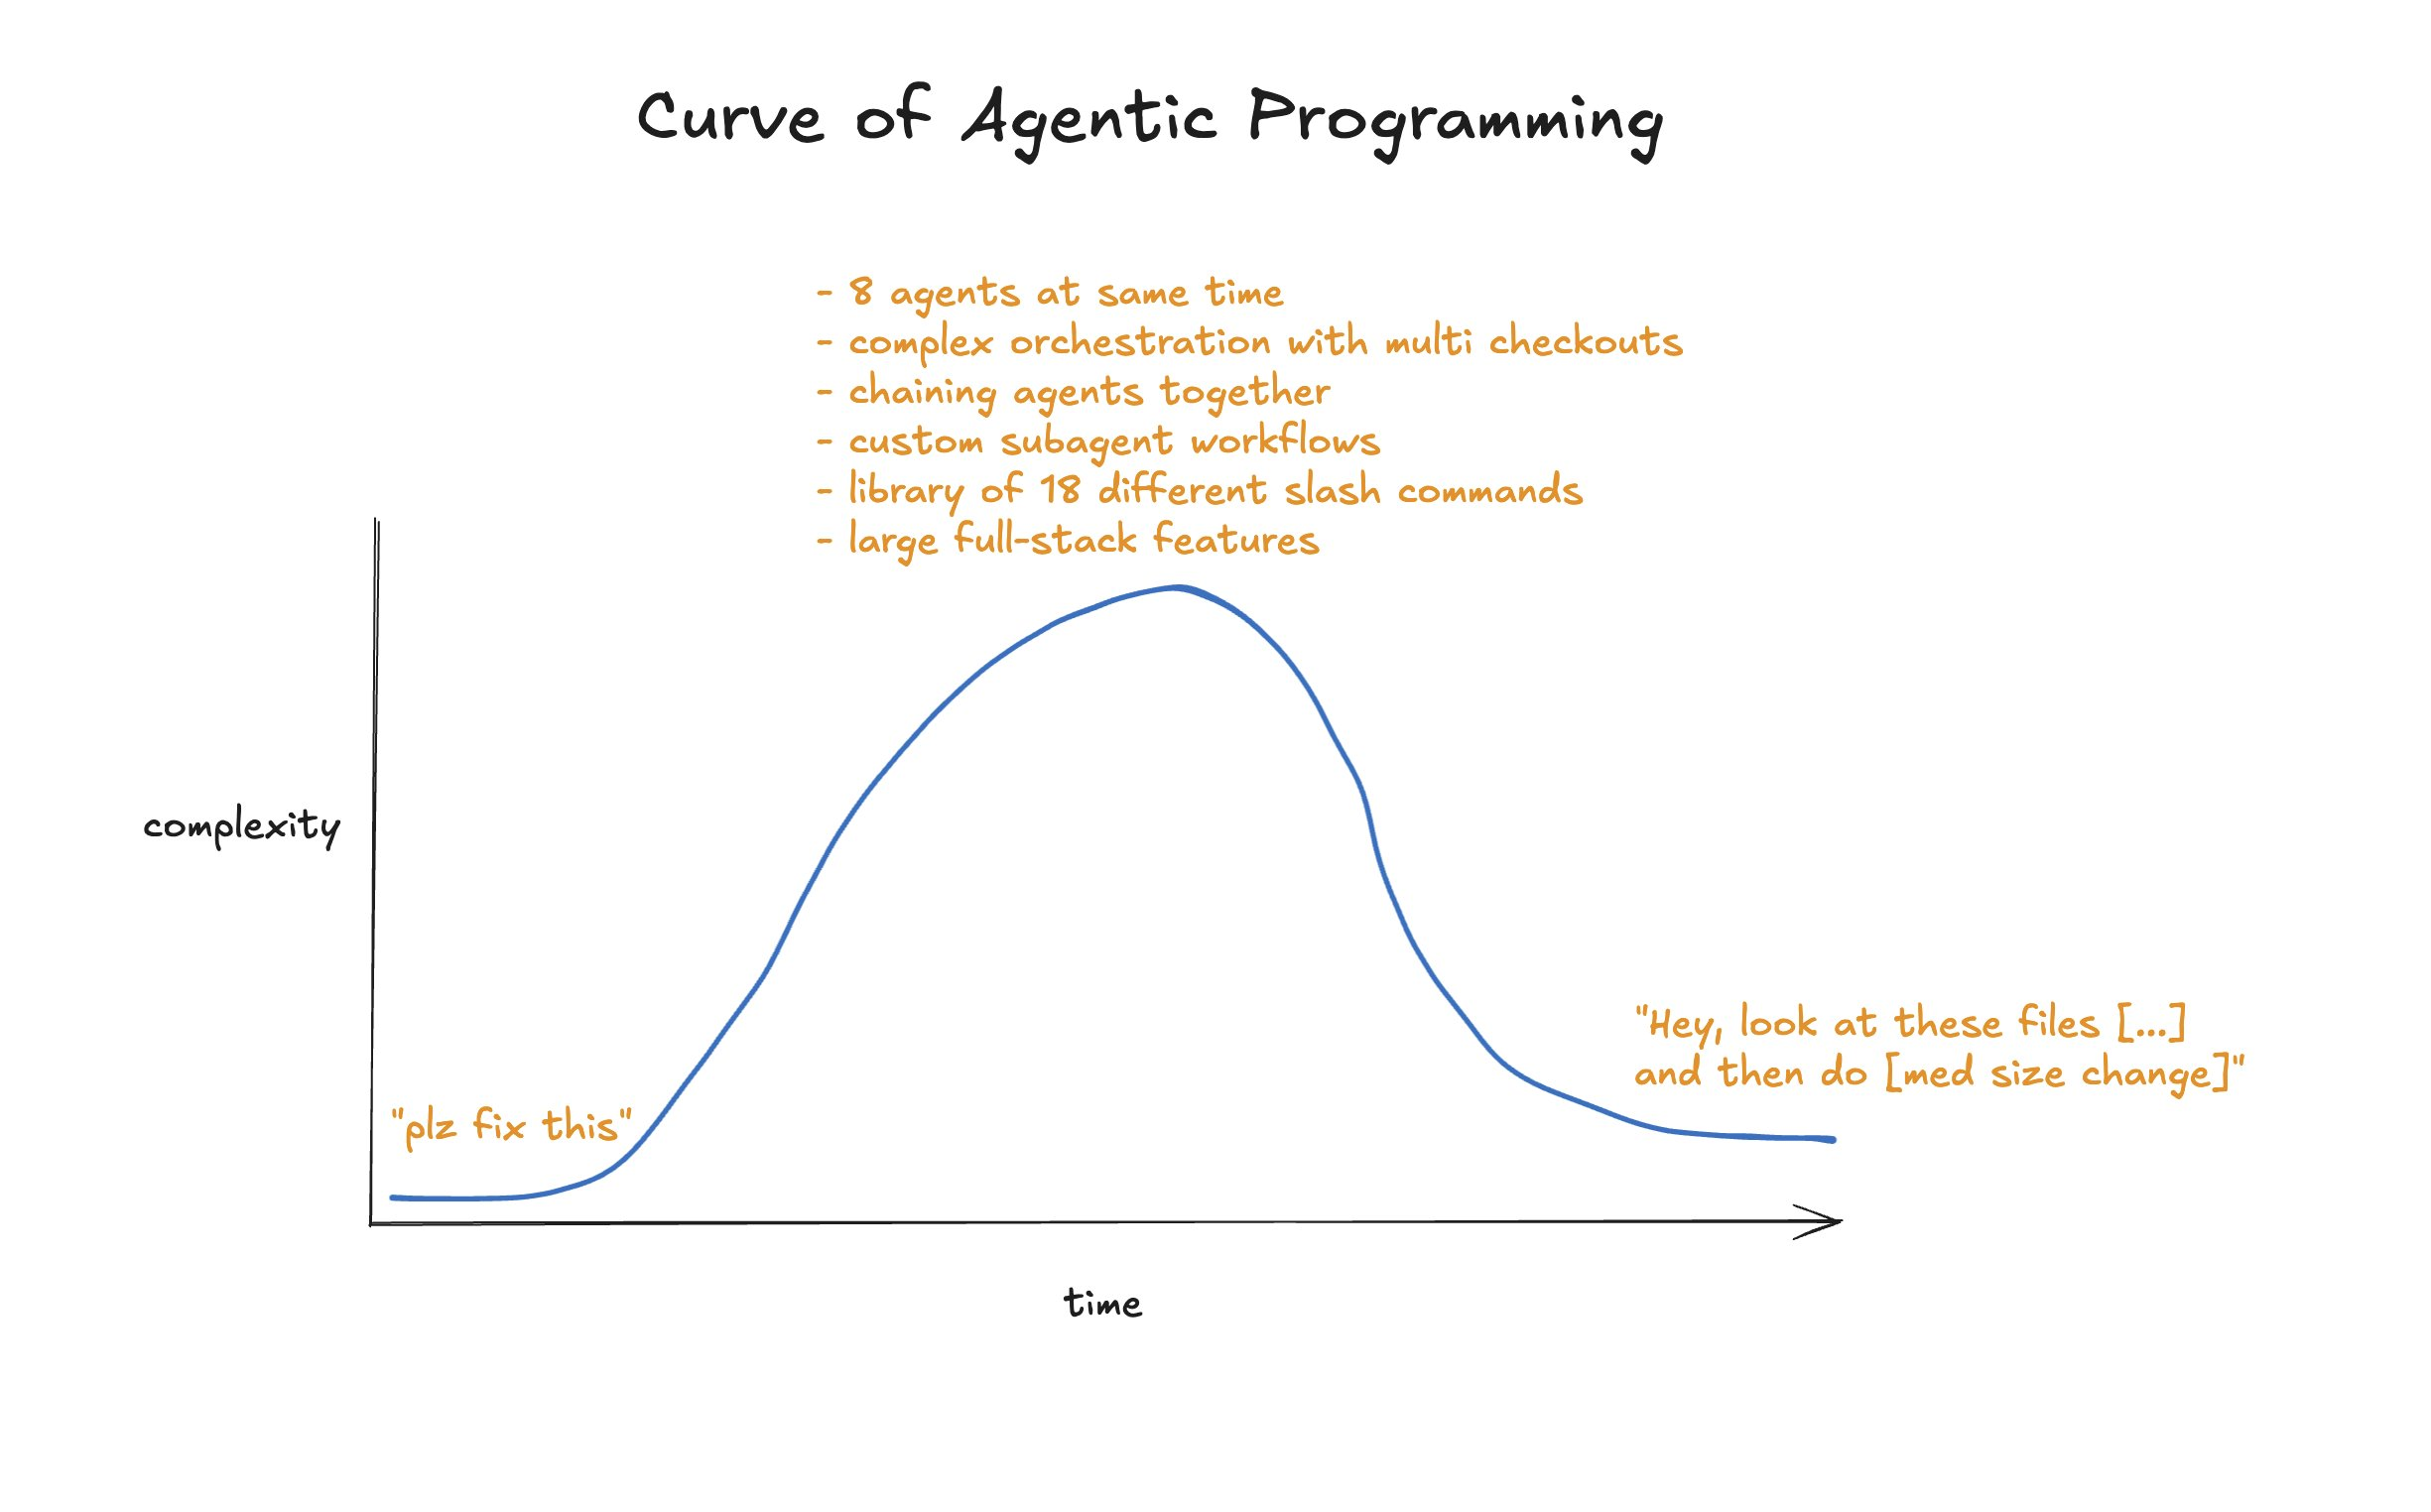
\includegraphics[height=0.68\textheight, width=\textwidth, keepaspectratio]{steipete-curve.jpg}

    \vspace{0.3em}
    {\tiny Peter Steinberger [7]}
\end{center}
\end{frame}

% TODO: demo slides for Principle 1


% =============================================
% SECTION 2: ASK PLAINLY AFTER YOU'VE THOUGHT
% =============================================
\begin{frame}{\#2: Ask Plainly After You've Thought}
Once the thinking is clear, the input can be simple.

\vspace{0.8em}
Frontier and even basic AI models are very capable of parsing and understanding your text better than complex prompt engineering.


\break
\pause
What people refer to as prompt engineering, in my opinion, can NEVER be generalised. It's all about context of the field and your specific role. Context that \textit{only} you have.



\break
\pause
If this could be automated and generalised, the frontier AI labs wouldn't be hiring more than ever.


\end{frame}

\begin{frame}
    \begin{center}
        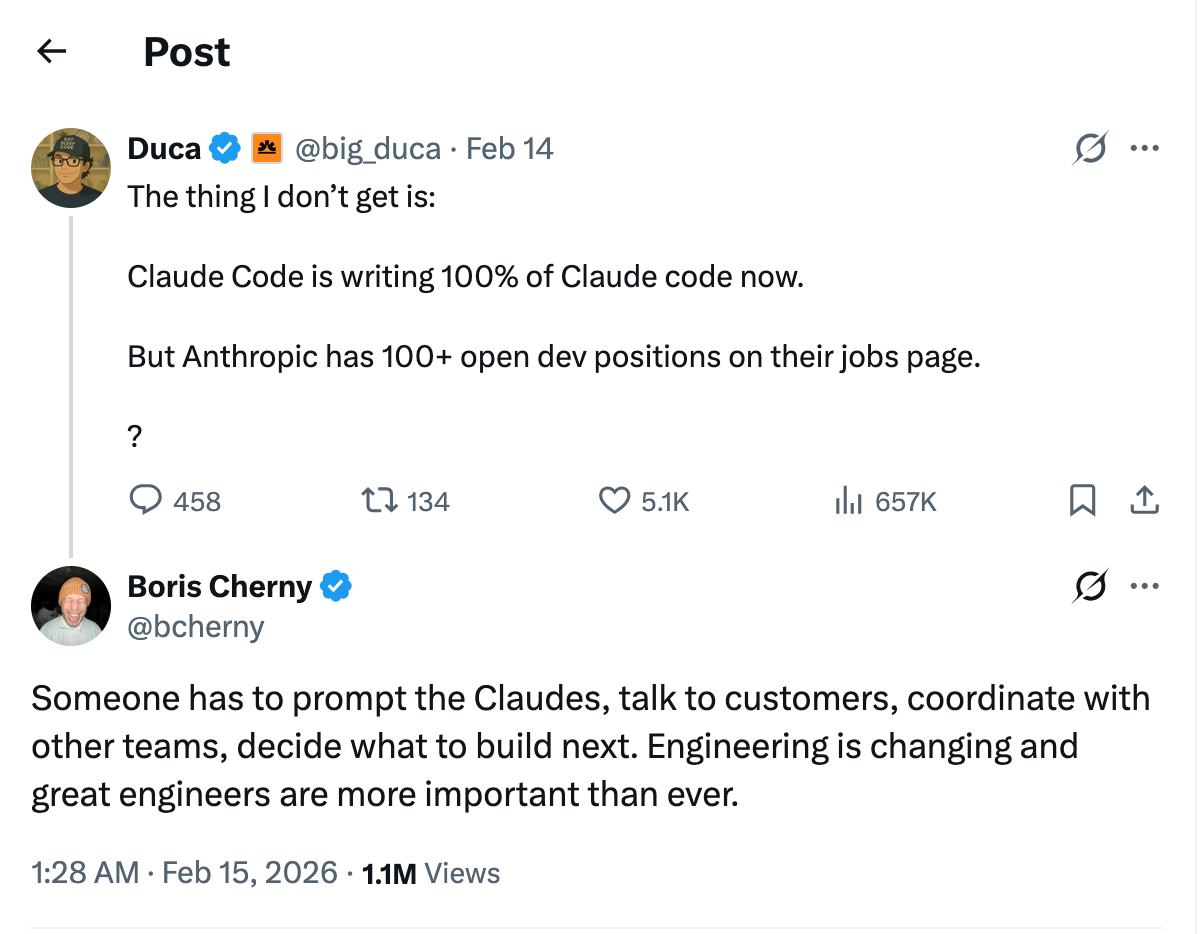
\includegraphics[height=0.66\textheight, keepaspectratio]{anthropic-engineers.png}

        \vspace{1em}
        {\tiny Boris Cherny on X [13]}
    \end{center}
\end{frame}

\begin{frame}{\#2: Ask Plainly After You've Thought}


This is great news! It means your job is more secure than you thought. It also means all roles are evolving closer into product roles.

\break
Describe what you want like you'd tell a colleague using direct and simple language, and iterate from there. (More on that in \#3.)

\vspace{0.8em}

\vspace{0.8em}
\textit{Clear thinking first. Plain speech second.}
\end{frame}

\begin{frame}
    \begin{center}
        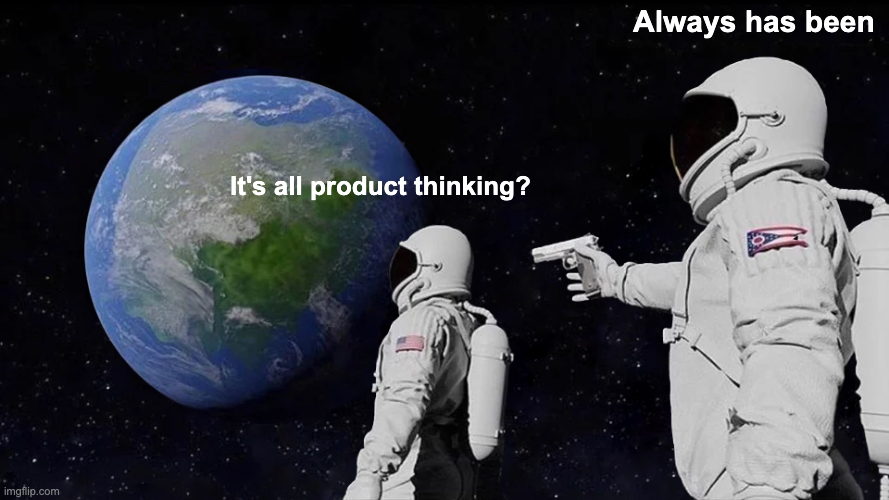
\includegraphics[height=0.66\textheight, keepaspectratio]{product-thinking-always-has-been.png}
    
        \vspace{2em}
        {\tiny This one's an original, no reference. Why're you still reading this?}
    \end{center}
\end{frame}

% =============================================
% SECTION 3: READ EVERYTHING YOU SHIP / RESPECT YOUR READER
% =============================================
\section{Respect Your Reader}

\begin{frame}{\#3: Read Everything You Ship}
The problem used to be the first draft. It used to take time.

\pause
\vspace{0.8em}
But Gen AI has lowered the barrier to entry - and things are now 10-20x faster than they were before.
This is true of code, specs, emails, anything.


\pause
\vspace{0.8em}
\textit{Writing is a product - and good writing means having empathy for your reader. It's all product design.}
\end{frame}

% TODO: demo slides for Principle 2


\begin{frame}{\#3: Read Everything You Ship}
\framesubtitle{Respect Your Reader}
\small
Writing has never been the hardest part of the process - reading is. A
You cannot communicate something until you understand it, and AI can never own this part of the process. Only you can.

\pause
\vspace{0.8em}
Good writing must involve understanding what your reader has in mind. That is your \textit{core work}.

\break
\pause
\tiny
\vspace{0.8em}
This problem predates AI but has been exacerbated by it. And it erodes trust. 54\% of people who received unreviewed AI output viewed the sender as less creative, and 42\% as less trustworthy [8].

\pause
\normalsize
\vspace{0.4em}
\textit{Your core work isn't the writing itself, but what the writing accomplishes and who can understand it. Good writing takes time!}
\end{frame}

\begin{frame}
    \begin{center}
        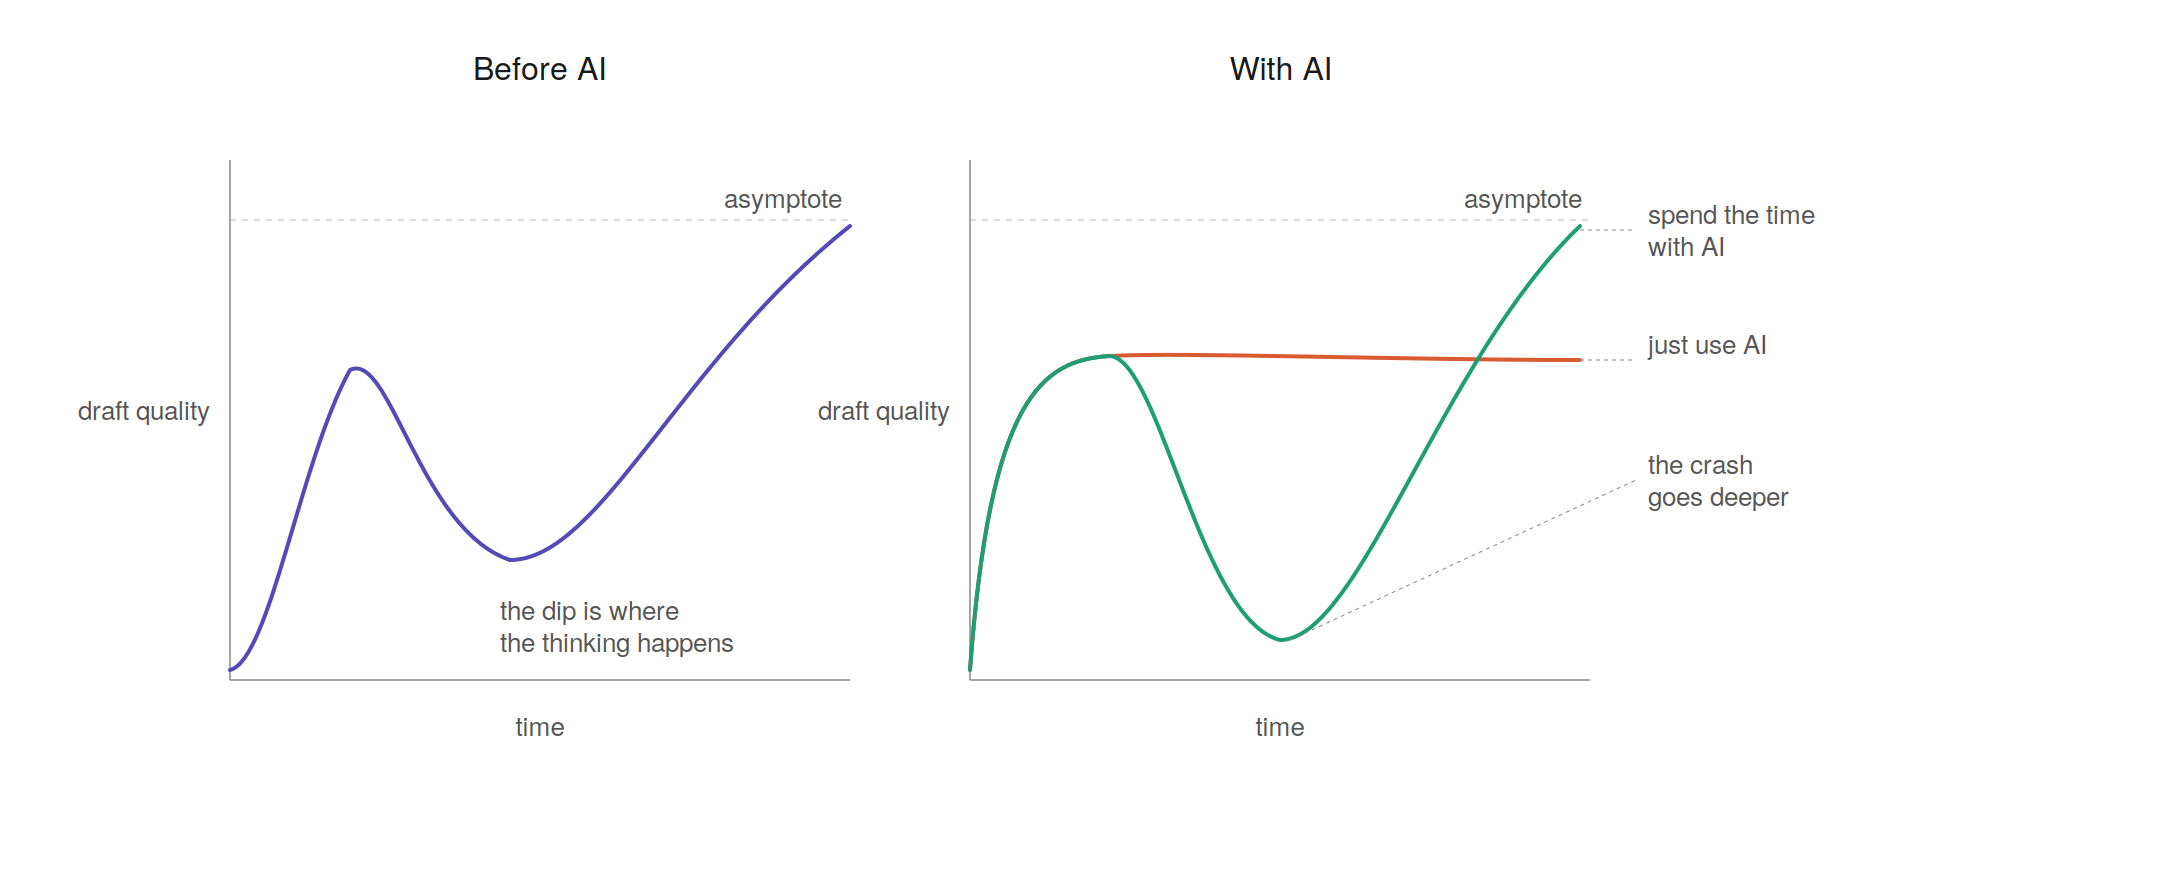
\includegraphics[width=0.92\textwidth, trim=80 20 220 40, clip]{writing_vs_reading.png}

        \vspace{2em}
        {\tiny This one's an original as well. Your core work is often navigating that crash, with or without AI.}
    \end{center}
\end{frame}

% TODO: demo slides for Principle 3

\section{Practical Tips}
\begin{frame}{Practical Tips Cheat Sheet}
\footnotesize
    \begin{enumerate}
        \pause
        \item Start your sketching on pen-and-paper (or a blank doc - no AI). It's almost always more unencumbered there.
        \pause
        \item As and when something works, write it down in an md file and keep these snippets handy.
        \pause
        \item Use the coding desktop apps in the folders. You don't need to be a coder!
        \pause
        \item Control the scaffolding. Come up with the skeleton yourself! That's something often only you can do. Do good old-fashioned google searches and read real examples when possible.
        \pause
        \item For coders, this means: Generate templates and folders using the package manager and not AI. AI regularly screws up there.
    \end{enumerate}


\vspace{0.6em}
\pause
Above all else, be curious. Read and explore. Ask lots of questions and share what you learn! \textit{(Slack: \#technical-support)}
    
\end{frame}

% =============================================
% CLOSE
% =============================================
\section{Close}

\begin{frame}{Contradictions}
Some of what makes you uneasy about AI isn't in your head.

\vspace{1em}
\begin{itemize}
    \item Code is cheaper to generate [11], but not cheaper to own. 
    \item Fast output can still create real costs: compute, oversight, and technical debt.
    \item Labour-saving tools can also raise standards and expectations [9].
\end{itemize}

\vspace{1em}
\textit{The question isn't whether AI makes work faster. It's what else comes with that speed.}
\end{frame}

\begin{frame}{Contradictions}
\small
A BCG study of 1,488 workers (March 2026) found [12]:
\begin{itemize}
    \item Heavy AI oversight $\rightarrow$ 14\% more mental effort, 33\% more decision fatigue
    \item Workers described "buzzing," mental fog, slower thinking
    \item But: using AI to replace repetitive tasks reduced burnout by 15\%
\end{itemize}

\vspace{0.8em}
Technologies sold as time-saving often end up extending and intensifying work [10].

\vspace{0.8em}
\textit{There is a cognitive load to using AI, and these are innate contradictions to this set of emerging technologies.}
\end{frame}

\begin{frame}{What I'd Hope You Take With You}
\begin{itemize}
    \item Think first, then delegate.
    \item Ask plainly after you've thought.
    \item Read everything you ship.
\end{itemize}

\vspace{1em}
And accept that there are contradictions.

\vspace{0.8em}
AI can make work faster and stranger at the same time.
Useful and exhausting. Powerful and costly.

\vspace{0.8em}
\textit{The goal is not to resolve all of that. It's to work with it more deliberately.}
\end{frame}

\begin{frame}{Stay In Touch}
\begin{center}
\small
{\footnotesize Link to presentation:}

{\tiny \url{https://github.com/dsih-artpark/workshops/blob/main/workshops/workshop-02-gen-ai-workflows-01/presentation.pdf}}

\vspace{1.6em}
Reach out if you have workflows you'd like to share.

\vspace{0.8em}
Future workshops are dependent on your interest.

\vspace{1.2em}
\textbf{Slack Channel: \#technical-support}

\vspace{0.6em}
Or DM.
\end{center}
\end{frame}


% =============================================
% UPCOMING WORKSHOPS
% =============================================
\begin{frame}{Coming Up}
Different team members can take up different workshop themes next:

\vspace{1em}
\begin{enumerate}
    \item Advanced Experiment Tracking \& Documentation (with gen AI powered workflows)
    \pause
    \item Practically Demystifying Code Generation tools and Concepts (like Skills, MCP, harnesses)
    \pause
    \item Writing and Implementing Engineering Specs, Project Tooling when using Code Gen
\end{enumerate}
\end{frame}


% =============================================
% REFERENCES
% =============================================
\section{References}

\begin{frame}{References \& Reading}
\tiny
\raggedright
\sloppy
\Urlmuskip=0mu plus 2mu\relax
[1] Fosslien L (2024) The AI adoption curve often involves an emotional spiral [LinkedIn post]. LinkedIn. Available: \url{https://www.linkedin.com/posts/liz-fosslien_the-ai-adoption-curve-often-involves-an-emotional-activity-7449860022924185600-Q2PZ/}. Accessed 2026 Apr 15.

\vspace{0.6em}
[2] Majic Predin J (2026) How To Get A Company AI Pilled And What VCs Want To See Next. Forbes. Available: \url{https://www.forbes.com/sites/josipamajic/2026/04/09/how-to-get-a-company-ai-pilled-and-what-vcs-want-to-see-next/}. Accessed 2026 Apr 15.

\vspace{0.6em}
[3] Palmer A (2025) Shopify CEO says staffers need to prove jobs can't be done by AI before asking for more headcount. CNBC. Available: \url{https://www.cnbc.com/2025/04/07/shopify-ceo-prove-ai-cant-do-jobs-before-asking-for-more-headcount.html}. Accessed 2026 Apr 15.

\vspace{0.6em}
[4] Morales J (2026) Amazon calls upon senior engineers to address issues created by ``Gen-AI assisted changes'', report claims. Tom's Hardware. Available: \url{https://www.tomshardware.com/tech-industry/artificial-intelligence/amazon-calls-engineers-to-address-issues-caused-by-use-of-ai-tools-report-claims-company-says-recent-incidents-had-high-blast-radius-and-were-allegedly-related-to-gen-ai-assisted-changes}. Accessed 2026 Apr 15.

\vspace{0.6em}
[5] BetterUp Labs (2025) Workslop: The hidden cost of AI-generated busywork. BetterUp. Available: \url{https://www.betterup.com/workslop}. Accessed 2026 Apr 15.
\end{frame}

\begin{frame}{References \& Reading}
\tiny
\raggedright
\sloppy
\Urlmuskip=0mu plus 2mu\relax
[6] Alpert S (2024) Everyone is wrong about that Slack flowchart. Sophie Alpert. Available: \url{https://sophiebits.com/2024/10/30/everyone-is-wrong-about-that-slack-flowchart}. Accessed 2026 Apr 15.

\vspace{0.6em}
[7] Steinberger P (2024) Just talk to it. steipete. Available: \url{https://steipete.me/posts/just-talk-to-it}. Accessed 2026 Apr 15.

\vspace{0.6em}
[8] Niederhoffer K, Robichaux A, Hancock JT (2026) Why People Create AI ``Workslop''-and How to Stop It. Harvard Business Review. Available: \url{https://hbr.org/2026/01/why-people-create-ai-workslop-and-how-to-stop-it}. Accessed 2026 Apr 15.

\vspace{0.6em}
[9] Cowan RS (1983) More Work for Mother: The Ironies of Household Technology from the Open Hearth to the Microwave. New York: Basic Books.

\vspace{0.6em}
[10] Wajcman J (2018) Digital technology, work extension and the acceleration society. German Journal of Human Resource Management. Available: \url{https://journals.sagepub.com/doi/10.1177/2397002218775930}. Accessed 2026 Apr 15.

\vspace{0.6em}
[11] Nadh K (2026) Code is cheap. Show me the talk. nadh.in. Available: \url{https://nadh.in/blog/code-is-cheap/}. Accessed 2026 Apr 15.

\vspace{0.6em}
[12] Bedard J, Kropp M, Hsu M, Karaman OT, Hawes J, Rosen Kellerman G (2026) When Using AI Leads to ``Brain Fry''. Harvard Business Review. Available: \url{https://hbr.org/2026/03/when-using-ai-leads-to-brain-fry}. Accessed 2026 Apr 15.

\vspace{0.6em}
[13] Cherny B (2026) Post on X. Available: \url{https://x.com/bcherny/status/2022762422302576970}. Accessed 2026 Apr 16.
\end{frame}

\end{document}
